
\section{NIO network implementation impact on performance}

Maciej and Tadek extended JPaxos by new implementation of Network module -- NIO. They expected NIO to be faster than 'old' java IO (which we call TCP, despite both Network modules using TCP). These tests show if it was worth writing.

\subsection{1024B requess -- network saturation}

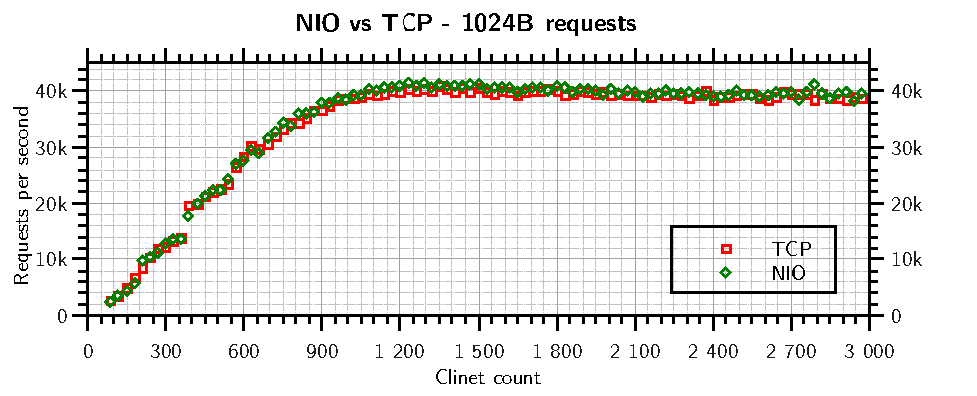
\includegraphics{tcp_nio/tcp_nio_1024}

NIO throughput is 'a little better' -- on average higher by 0,7\%. The trend is identical.

\subsection{128B requess -- CPU saturation}

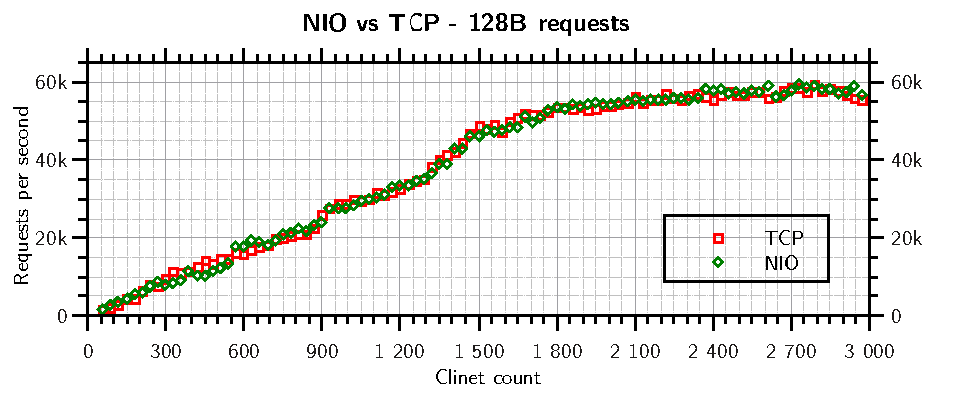
\includegraphics{tcp_nio/tcp_nio_128}

Here, the CPU is more saturated. NIO was meant to help in such case. The experiments however do not agree with this claim -- NIO and 'old IO' perform the same (NIO is on average 0,3\% slower).

\paragraph{Conclusion} it makes no real difference for JPaxos whether it uses NIO or 'old IO'.